\documentclass{article}
\usepackage{tikz}
\usetikzlibrary{graphs,graphdrawing}
\usepackage{caption}

\usepackage{multirow}
\usepackage{multicol}
\usepackage[framemethod=tikz]{mdframed}
\usepackage{lipsum}
\usepackage{tkz-graph}
\usegdlibrary{trees}
\usepackage{amsmath, amssymb}
\usepackage{pst-node}
\usepackage{blkarray}
\usepackage{amsmath, amssymb}
\usepackage{pst-node}

\usepackage[margin=2cm]{geometry}

\usepackage[utf8]{inputenc}
\begin{document}
	\section{Esercitazione 5}
	\subsection{Esercizio 1}

	Una industria produttrice di videoregistratori è talmente sicura della qualità dei propri prodotti da
	garantire per due anni la sostituzione dell’apparecchio in caso di guasto; le statistiche dell’azienda
	indicano che soltanto l’1\% dei videoregistratori si guasta durante il primo anno ed il 5\% durante il
	secondo. La garanzia non copre gli apparecchi forniti in sostituzione di quelli guasti. Formulare il
	problema come una catena di Markov, fornendo la matrice di transizione.
	
	Innanzitutto dobbiamo chiarire quali sono gli stati del sistema;
	Immaginiamo di rappresentare la vita del videoregistratore in quattro stati:
	\begin{enumerate}
		\item Stato $S_0$: quando il videoregistratore nuovo
		\item Stato $S_1$: quando il videoregistratore non è mai stato guasto nel primo anno
		\item Stato $S_2$: quando il videoregistratore è uscito da garanzia
		\item Stato $S_3$; quando il videoregistratore è guasto e sostituito.
	\end{enumerate}

A questo punto possiamo creare la matrice di transizione:

\[
T = 
\begin{blockarray}{ccccc}
	  & S_0 & S_1 & S_2 & S_3 \\
	\begin{block}{c(cccc)}
		S_0 & 0 & 0.99 & 0 & 0.01 \\
		S_1 & 0 & 0 & 0.95 & 0.05 \\
		S_2 & 0 & 0 & 1 & 0 \\
		S_3 & 0 & 0 & 0 & 1 \\
	\end{block}
\end{blockarray}
\]

	\subsection{Esercizio 2}
	Consideriamo la catena di Markov su 
	$E = {1,2,3,4}$ associata alla matrice di transizione
\[
P = 
\begin{blockarray}{ccccc}
	 & S_1 & S_2 & S_3 & S_4 \\
	\begin{block}{c(cccc)}
	 S_1 &	0.25 & 0   & 0.75 & 0 \\
	 S_2 &	0.25 & 0.5 & 0.25 & 0 \\
	 S_3 &	0.5  & 0   & 0.5  & 0 \\
	 S_4 &	0    & \frac{1}{3} &  \frac{1}{3} &  \frac{1}{3} \\
	\end{block}
\end{blockarray}
\]	

\begin{itemize}
	\item Qual è la probabilità partendo da $S_2$ di essere ancora in $S_2$ dopo due passi?
\end{itemize}

\pagebreak
\begin{mdframed}[hidealllines=true,backgroundcolor=blue!20]
	Se una catena di markov è in uno stato $i$ al tempo $m$, qual è la probabilità che dopo $n$ passi sarà in uno stato $j$?
	
	Per definizione sappiamo che in una catena di markov è vero che:
	
	\[
		P(X_{m + n} = j | X_m = i) = P(X_{n} = j | X_0 = i) = P_{ij}(n)
	\]
	Ovvero che la probabilità di passare allo stato $j$ in $n$ passi partendo dallo stato $i$ al passo $m$ è uguale alla probabilità di passare allo stato $j$ in $n$ passi partendo dallo stato $i$ al tempo $0$.
	
	Chiamiamo questa probabilità $P_{ij}(n)$.
	
	Partiamo dal caso più semplice, quello in cui ci sono due passaggi fra lo stato $i$ e lo stato $j$.
	
	Necessariamente avremo che ci sarà uno stato intermedio $k$, che non è conosciuto.
	
	Avremo quindi che la possibilità di passare da $i$ a $j$ in due passaggi sarà data dalla sommatoria di tutte le probabilità $p_{ik} \cdot p_{kj}$ per tutti i possibili stati intermedi $k$.
	
	\[
		P_{ij}(2) = \sum_{k=1}^{n} p_{ik} \cdot p_{kj}
	\]
	
	Nell'esempio della cola visto a lezione si avrebbe ad esempio che per passare a cola 1 da cola 2 in 2 passi il risultato sarebbe:
	
	
	\[
	P = 
	\begin{blockarray}{ccc}
		& Cola  1 & Cola 2 \\
		\begin{block}{c(cc)}
			Cola 1  &  0.9   & 0.1 \\
			Cola 2  &  0.2   & 0.8 \\
		\end{block}
	\end{blockarray}
	\]
	
	\[
	 P_{Cola \; 1\; Cola 2}(2) = P_{Cola1 \; Cola1} * P_{Cola1 \; Cola2} + P_{Cola1 \; Cola2} * P_{Cola2 \; Cola2} = 
	 0.9 * 0.1 + 0.1 * 0.8 = 0.17
	\]
	
	Notiamo però che l'operazione di sommatoria fra tutti i percorsi intermedi equivale a fare un prodotto riga per colonna della matrice per sè stessa, pertanto possiamo concludere che
	
	$P_{ij}(2)$ è uguale all'elemento in posizione $i,j$ della matrice $P^2$
	
	Questo ragionamento può essere esteso a potenze maggiori di due;
	
	In generale se la probabilità che una catena di Markov sia in uno stato j dopo n passi, partendo dallo stato i è:
	
	\[
		P_{ij}(n)
	\]
	Ovvero l'ij-simo elemento di $P^n$
\end{mdframed}


Formalmente la richiesta è trovare $P_{2,2}^{(2)}$, che per definizione è uguale a $(P^2)_{2,2}$.

Quando consideriamo la matrice $P^2$ consideriamo la matrice che per ogni cella ci dice qual è la probabilità di finire in uno stato dato lo stato precedente.

In particolare nel nostro caso vogliamo solo la posizione $2,2$ .

Possiamo quindi fare il prodotto riga per colonna della seconda riga per la seconda colonna:

\[
(P^2)_{2,2} = \sum_{h} P_{2,h} \cdot P_{h,2} = (0.25 \cdot 0) + (0.5 \cdot 0.5) + (0.25 \cdot 0) + (0 \cdot \frac{1}{3}) = \frac{1}{4}
\]
\pagebreak

\begin{itemize}
	\item Qual è la probabilità partendo da $S_3$ di essere ancora in $S_2$ dopo due passi?
\end{itemize}

La richiesta formalmente è Formalmente la richiesta è trovare $P_{3,2}^{(2)}$, che per definizione è uguale a $(P^2)_{3,2}$.


Avremo quindi che:

\[
(P^2)_{2,2} = \sum_{h} P_{2,h} \cdot P_{h,2} = (0.25 \cdot 0) + (0.5 \cdot 0.5) + (0.25 \cdot 0) + (0 \cdot \frac{1}{3}) = \frac{1}{4}
\]

Andiamo quindi a calcolare

\[
\sum_{h} P_{3,h} \cdot P_{h,2}  
\]

Che è il prodotto riga per colonna della terza riga per la seconda colonna, ovvero

\[
 = (0.5 \cdot 0 ) + (0 \cdot 0.5) + (0.5 \cdot 0) + (0 \cdot \frac{1}{3} ) = 0
\]

\begin{itemize}
	\item Qual è la probabilità di essere in $S_2$ partendo da $S_2$ dopo 12 passi?
\end{itemize}

La richiesta equivale a calcolare $P_{2,2}^{(12)}$.

Dovremmo fare molti calcoli, ma possiamo fare alcuni considerazioni: dopo alcune iterazioni l'unico modo che ho di rientrare in $S2$ è passare da sè stesso, per cui la probabilità sarà $P_{2,2}^{(12)} = 0.5^{12}$

\pagebreak
\subsection{Esercizio 3}

Consideriamo al catena di markov sui vertici di un tringolo equilatero definita dalle regole seguenti: ad ogni istante essa si può spostare da un vertice a quello adiacente in senso antiorario con probabilità $p$ e in senso orario con probabilità $1-p$, dove $0<p<1$

\begin{center}
	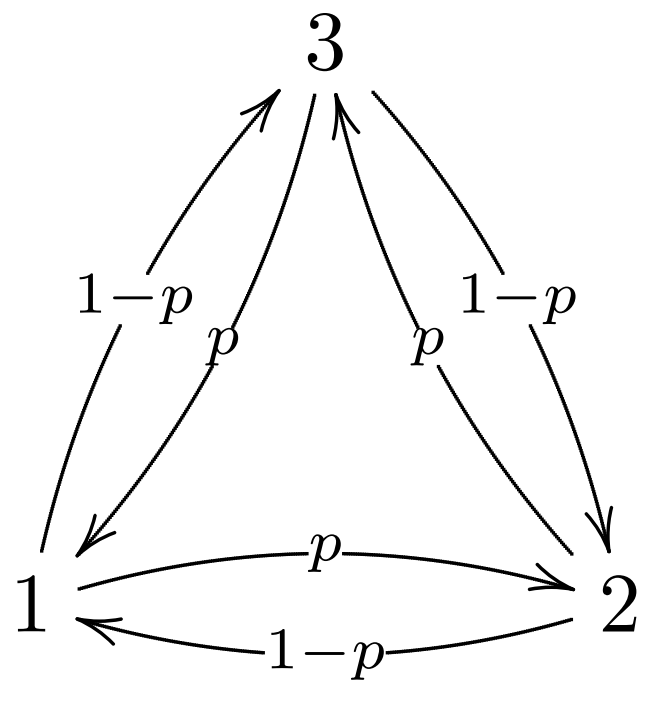
\includegraphics[width=4cm]{./immagini/es5}
\end{center}
\[
T = 
\begin{blockarray}{cccc}
	& 1 & 2 & 3 \\
	\begin{block}{c(ccc)}
		1 &	0     & $p$   & $1-p$ \\
		2 &	$1-p$ & 0     &  $p$  \\
		3 &	$p$  & $1-p$   & 0  \\
	\end{block}
\end{blockarray}
\]

\begin{itemize}
	\item La catena di Markov è regolare?
\end{itemize}

\begin{mdframed}[hidealllines=true,backgroundcolor=blue!20]
	Che cosa significa dire che una catena di Markov è regolare? \\
	Significa che esiste un intero positivo maggiore di 1 $k$ tale per cui l'elevamento a potenza della matrice delle probabilità $P$ alla $k$ risulti strettamente maggiore di 0. 
	
	\[ \exists k > 1  \; | \;  T^{k} > 0 \]
	
	Ovvero nella matrice finale non ho nessuno 0: un qualunque stato è raggiungibile da un qualunque altro stato.
\end{mdframed}

Se eleviamo la matrice $T$ alla seconda notiamo che nessun valore è uguale a 0, per cui possiamo dire che la catena di Markov è regolare.

La matrice $T^{2}$:

\[
T^2 = 
\begin{blockarray}{cccc}
	& 1 & 2 & 3 \\
	\begin{block}{c(ccc)}
		1 &	-2p^2 + 2p    & p^2 -2p + 1   & p^2 \\
		2 &	p^2           & -2p^2 + 2p    & p^2 -2p + 1  \\
		3 &	p^2 -2p + 1   & p^2           & -2p^2 + 2p  \\
	\end{block}
\end{blockarray}
\]

Dobbiamo quindi valutare le seguenti espressioni:
\begin{itemize}
	\item $p^2 > 0$ \\
	Sappiamo dal testo che $0 < p < 1$, per cui $p^2$ sarà sempre > 0
	\item $-2p^2 + 2p$ \\
	Abbiamo che:
	\[
		-2p^2 + 2p > 0 = -p^2 + p > 0 = p^2 -p < 0 = p(p-1) < 0
	\]
	\[
	 0 < p < 1
	\]
	Che nel nostro caso è sempre vero
	\item $p^2 -2p + 1$ \\
	Abbiamo che
	\[
	p^2 -2p + 1 > 0 
	\]
	che è sempre > 0
\end{itemize}

\pagebreak
\subsection{Esercizio 4}

Un computer può operare in due modalità. Ogni ora, il computer rimane nella stessa modalità
oppure cambia modalità in accordo alla seguente matrice di probabilità di transizione
	\[
P = 
\begin{blockarray}{ccc}
	& S_1 & S_2 \\
	\begin{block}{c(cc)}
		S_1  &  0.4   & 0.6 \\
		S_2  &  0.6   & 0.4 \\
	\end{block}
\end{blockarray}
\]

\begin{itemize}
	\item Calcolare la probabilità di transizione a due step
\end{itemize}

È sufficente calcolare $P^2$
	\[
P^2 = 
\begin{blockarray}{ccc}
	& S_1 & S_2 \\
	\begin{block}{c(cc)}
		S_1  &  0.52   & 0.48 \\
		S_2  &  0.48   & 0.52 \\
	\end{block}
\end{blockarray}
\]

\begin{itemize}
	\item Se il sistema si trova nella modalità 1 alle 17:30, qual è la probabilità che esso si trovi nella
	modalità 1 alle 20:30?
\end{itemize}


Dobbiamo calcolare $P^{(3)}_{1,1}$, che equivale a calcolare $P^3_{1,1}$.

Avendo già a disposizione $P^2$ basterà fare il prodotto riga per colonna di $P^2$ per $P$.

Avremo quindi che $P^3_{1,1}$ sarà:

\[
	(0.52 \cdot 0.4 ) + (0.48 \cdot 0.6) = 0.496
\]

\pagebreak

\subsection{Esercizio 5}

Determinare la struttura della catena di Markov partendo dalla matrice $P$.
\[
P = 
\begin{blockarray}{ccccc}
	& S_0 & S_1 & S_2 & S_3 \\
	\begin{block}{c(cccc)}
			\vspace{0.1cm}
		S_0 &   0 &	\frac{7}{8} & \frac{1}{16}   & \frac{1}{16} \\
		\vspace{0.1cm}
		S_1 &   0 &	\frac{3}{4} & \frac{1}{8}    & \frac{1}{8} \\
		\vspace{0.1cm}
		S_2 &	0 & 0           & \frac{1}{2}    & \frac{1}{2} \\
		\vspace{0.1cm}
		S_3 &	1 & 0           &  0             &  0 \\
	\end{block}
\end{blockarray}
\]	

\begin{center}
	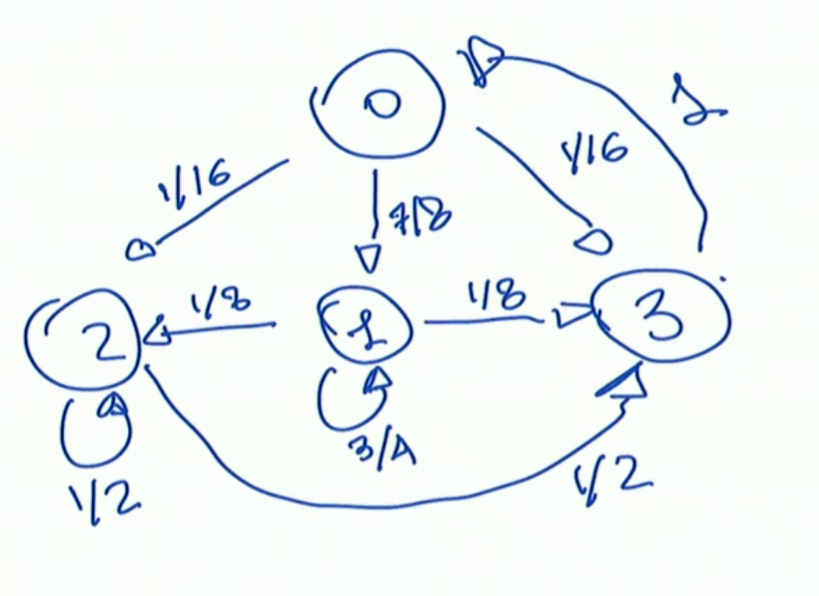
\includegraphics[width=10cm]{./immagini/es2}
\end{center}


\begin{itemize}
	\item Determinare lo stato stazionario
\end{itemize}

\begin{mdframed}[hidealllines=true,backgroundcolor=blue!20]
	Lo stato stazionario è quello stato in cui anche continuando a far evolvere il modello Markoviano (elevando ad una potenza superiore) la probabilità non cambia più.
\end{mdframed} 

Un modo per determinare i valori della matrice nello stato stazionario è quello di impostare un sistema di $n$ equazioni in $n$ incognite:

Dovrò mettere a sistema i quattro stati ponenodo che ogni stato sia in una situazione tale per cui la probabilità dello stato corrente è uguale a quella di tornare nello stato corrente con un ulteriore passo.

Ad esempio imponendo:
 \[\pi_0 = P_{00} \cdot \pi_0 + P_{10} \cdot \pi_{1} + P_{20} \cdot \pi_2 + P_{30} \cdot \pi_3
 \]

Stiamo imponendo che vogliamo uno stato stazionario $\pi_0$  tale che se si esegue uno step successivo la probabilità di trovarsi nello stato $\pi_0$ è la stessa da cui siamo partiti.


Dobbiamo anche garantire che gli stati finali siano una distribuzione stocastica, per cui aggiungiamo un'ultima equazione che garantisca che gli stati dello stato stazionario sommati diano 1.
\begin{equation}
	\begin{cases}
		\pi_0 = P_{00} \cdot \pi_0 + P_{10} \cdot \pi_{1} + P_{20} \cdot \pi_2 + P_{30} \cdot \pi_3 \\
		
		\pi_1 = P_{01} \cdot \pi_1 + P_{11} \cdot \pi_{1} + P_{21} \cdot \pi_{2} + P_{31} \cdot \pi_3 \\
		
		\pi_2 = P_{02} \cdot \pi_0 + P_{12} \cdot \pi_{1} + P_{22} \cdot \pi_{2} + P_{32} \cdot \pi_3 \\
		
		\pi_3  = P_{03} \cdot \pi_0 + P_{13} \cdot \pi_{1} + P_{23} \cdot \pi_{2} + P_{33} \cdot \pi_3 \\
		
		1 = \pi_{0} + \pi_{1} + \pi_{2} + \pi_{3} 
	\end{cases}\
\end{equation}

\pagebreak

Sostituendo con i valori noti otteniamo:
\begin{equation}
	\begin{cases}
		\pi_0 = 0 + 0 + 0 + 1 \cdot \pi_3 \\
		
		\pi_1 = \frac{7}{8} \cdot \pi_{0}  + \frac{3}{4} \cdot \pi_{1} + 0 + 0 \\
		
		\pi_2 = \frac{1}{16} \cdot \pi_{0}  + \frac{1}{8} \cdot \pi_{1} + \frac{1}{2} \cdot \pi_{2} + 0 \\
		
		\pi_3 = \frac{1}{16} \cdot \pi_{0}  + \frac{1}{8} \cdot \pi_{1} + \frac{1}{2} \cdot \pi_{2} + 0 \\
		
		
		1 = \pi_{0} + \pi_{1} + \pi_{2} + \pi_{3} 
	\end{cases}\
\end{equation}

Risolvendo il sistema otterremo che:

\[
\pi_{0} = \pi_{2} = \pi_{3} = \frac{2}{13}
\]

e che \[ \pi_{1} = \frac{7}{13} \]
\end{document}
